\documentclass{beamer}
\usetheme{CENIDETDIE}
\setbeamertemplate{caption}[numbered]
\usefonttheme[onlymath]{serif}

% ------------------------------------------------------------------------------------------------

\usepackage[utf8]{inputenc}
\usepackage[T1]{fontenc}
\usepackage{helvet}
\usepackage{graphicx} % Allows including images
\usepackage{booktabs} % Allows the use of \toprule, \midrule and \bottomrule in tables
\numberwithin{figure}{section}
\numberwithin{equation}{section}
\usepackage[square,sort,comma,numbers]{natbib}
\usepackage{ragged2e}
\usepackage{caption}
\usepackage{subcaption}
\usepackage{mathabx}

 

% ------------------------------------------------------------------------------------------------

\title{WORK PROGRESS}
%\subtitle{Presentation in Beamer-\LaTeX}
\author{Saeed ZAHRAN $^{1}$ }
\institute{$^{1}$UNIVERSITÉ DE PICARDIE JULES VERNE \\ 
		}
\date{\today}

\begin{document}

% ------------------------------------------------------------------------------------------------

\begin{frame}[plain,t]
\titlepage
\end{frame}

% ------------------------------------------------------------------------------------------------

% \begin{frame}[plain,noframenumbering]
%   \addtocounter{framenumber}{-1}
%   \scriptsize
%   \thispagestyle{empty}
%   \frametitle{Indice}
%   \setbeamertemplate{section in toc}[sections numbered]
%   \tableofcontents[hideallsubsections]
% \end{frame}

% ------------------------------------------------------------------------------------------------

% \section{RDF previous }
%  \frametitle{RDF previous }
%  \scriptsize
%   RDF was original writeen by Tim Bray in 1998 an update by Dan Brickley in 2001\cite{w3:2004:w3c}.\\ 
 %  \vspace{5mm}
 %  The Resource Description Framework (RDF) is a lenguage for representing information about resources in the World Wide Web\cite{w3:2004:w3c}.\\
%   \vspace{5mm}
%  RDF descriptions, often contain redundancies, and could be generated differently even when describing the same resources, which would have a negative impact on various RDF-based applications (e.g.,RDF storage, processing time, loading time, similarity measuring, mapping, alignment, and versioning)\cite{TiconaUltimo}.

% \end{frame}

% ------------------------------------------------------------------------------------------------

% \section{RDF definition}
% \begin{frame}
%  \frametitle{RDF definition}
 % 	\textbf{RDF graph:} set of triples 
 % 	\begin{figure}
  %       \centering
  %       \begin{subfigure}[h]{0.45\textwidth} 
   %          
\includegraphics[width=\textwidth]{pictures/rdf_begin}
   %          \label{fig:rdf_begin}
   %      \end{subfigure}       
    %     \begin{subfigure}[h]{0.45\textwidth} 
   %          
\includegraphics[width=\textwidth]{pictures/RDF_begin2}
   %          \label{fig:rdf_begin2}
   %      \end{subfigure}
    %     \caption{Example of RDF triple}
    % \end{figure}

 % 	\justify There can be three kinds of nodes: IRIs, literals, and blank nodes.
% 	\begin{itemize}
   %  \footnotesize
  %   \vspace{5mm}
  %   \item  \justify \textbf{IRI} (Internationalized Resource Identifier) refers to a resource (the referent).
  %   \item  \justify \textbf{Literal} denotes resources which have an associated value for example, an integer or string value.
  %   \item  \justify \textbf{Blank nodes} are local identifiers which do not identify specific resources.
% 	\end{itemize}

% \end{frame}

% ---------------------------------------------------------------------------------------
\section{}
\begin{frame}
 \frametitle{Gain Matrix}
 	%RDF data graph and RDF schema graph:
 	
 	\begin{figure}[p]
  		\centering
  		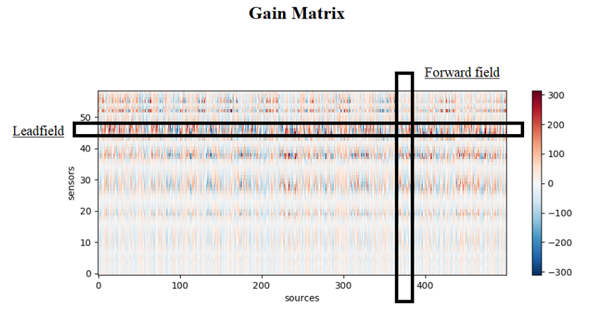
\includegraphics[width=1.0\linewidth]{pictures/lf}
  	%	\caption{\scriptsize Advantages of RDF summarization}
  		\label{fig:approaches_RDF}
 	\end{figure}
    
\end{frame}

% ------------------------------------------------------------------------------------------------

%------------------------------
\section{}
\begin{frame}
 \frametitle{MEG-Lambda max}
  

 	\begin{figure}[h]
        \begin{subfigure}[h]{0.53\linewidth} 
            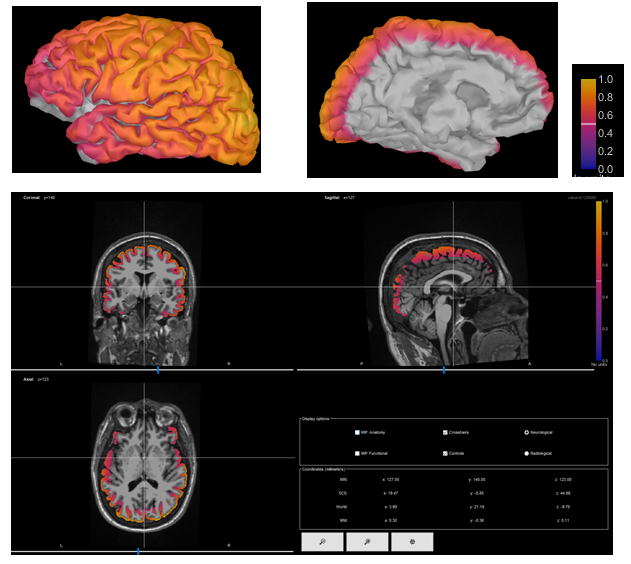
\includegraphics[width=\linewidth]{pictures/meg3}
           % \caption{\tiny RDF graph}
            \label{fig:rdf_graph}
        \end{subfigure}       
        \begin{subfigure}[h]{0.45\linewidth} 
            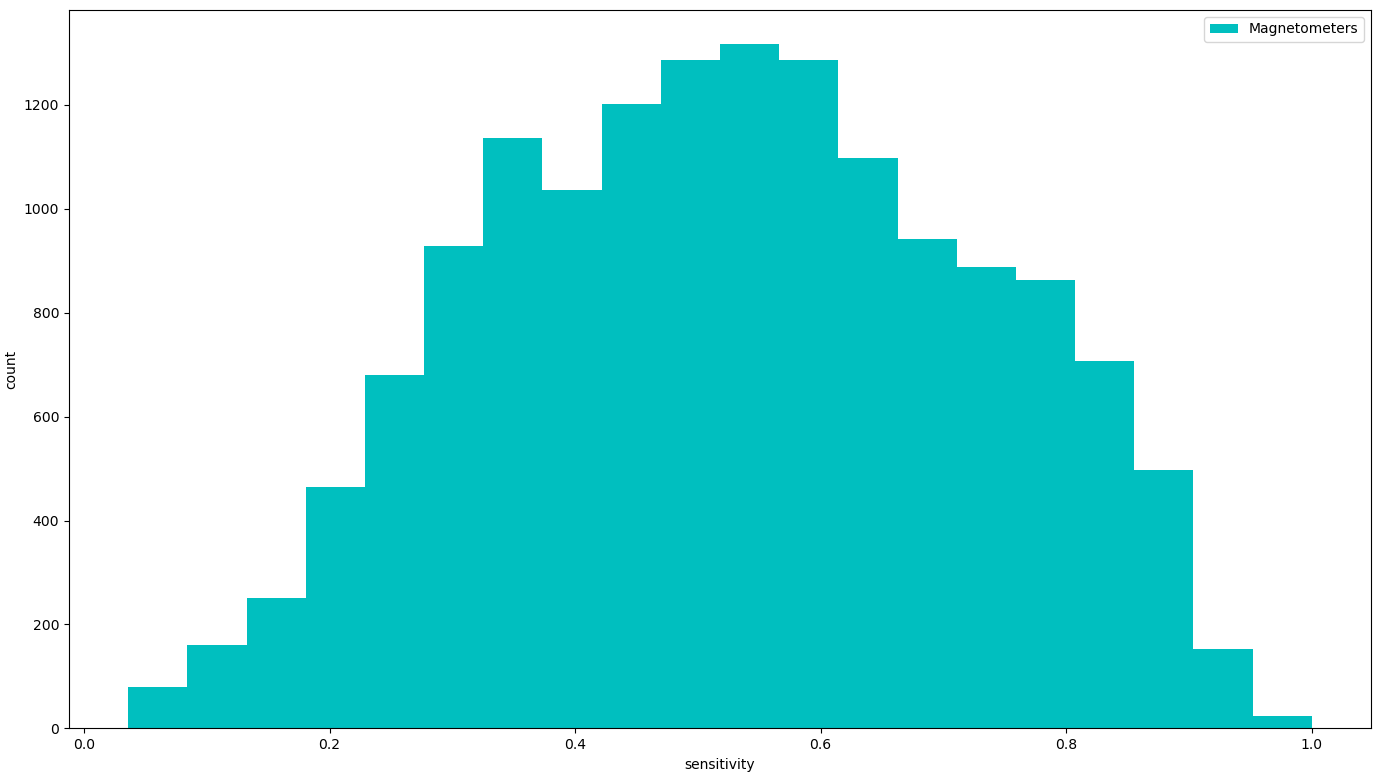
\includegraphics[width=\linewidth]{pictures/HISTmeg0.png}
           % \caption{\tiny RDF Shema (RDFS) graph}
            \label{fig:rdfs_graph}
        \end{subfigure}
       % \caption{\scriptsize Example of RDF graph and RDFS graph}
    \end{figure}

  
\end{frame}


%---------------
\section{}
\begin{frame}
 \frametitle{MEG-Lambda2 }
  

 	\begin{figure}[h]
        \begin{subfigure}[h]{0.53\linewidth} 
            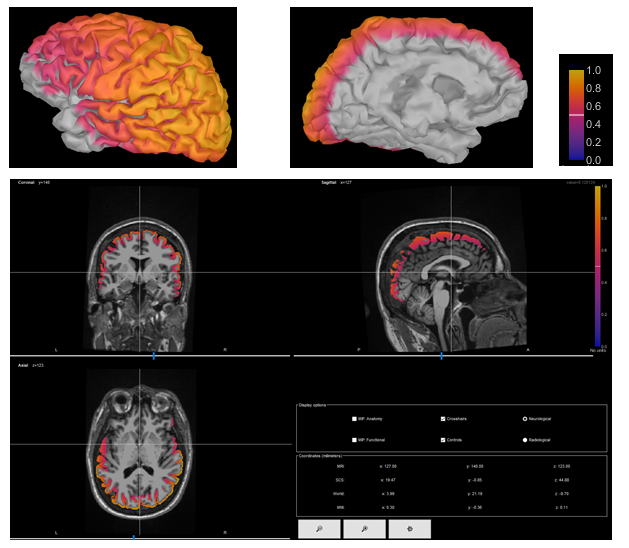
\includegraphics[width=\linewidth]{pictures/meg2}
           %  \caption{\tiny RDF graph}
            \label{fig:rdf_graph}
        \end{subfigure}       
        \begin{subfigure}[h]{0.45\linewidth} 
            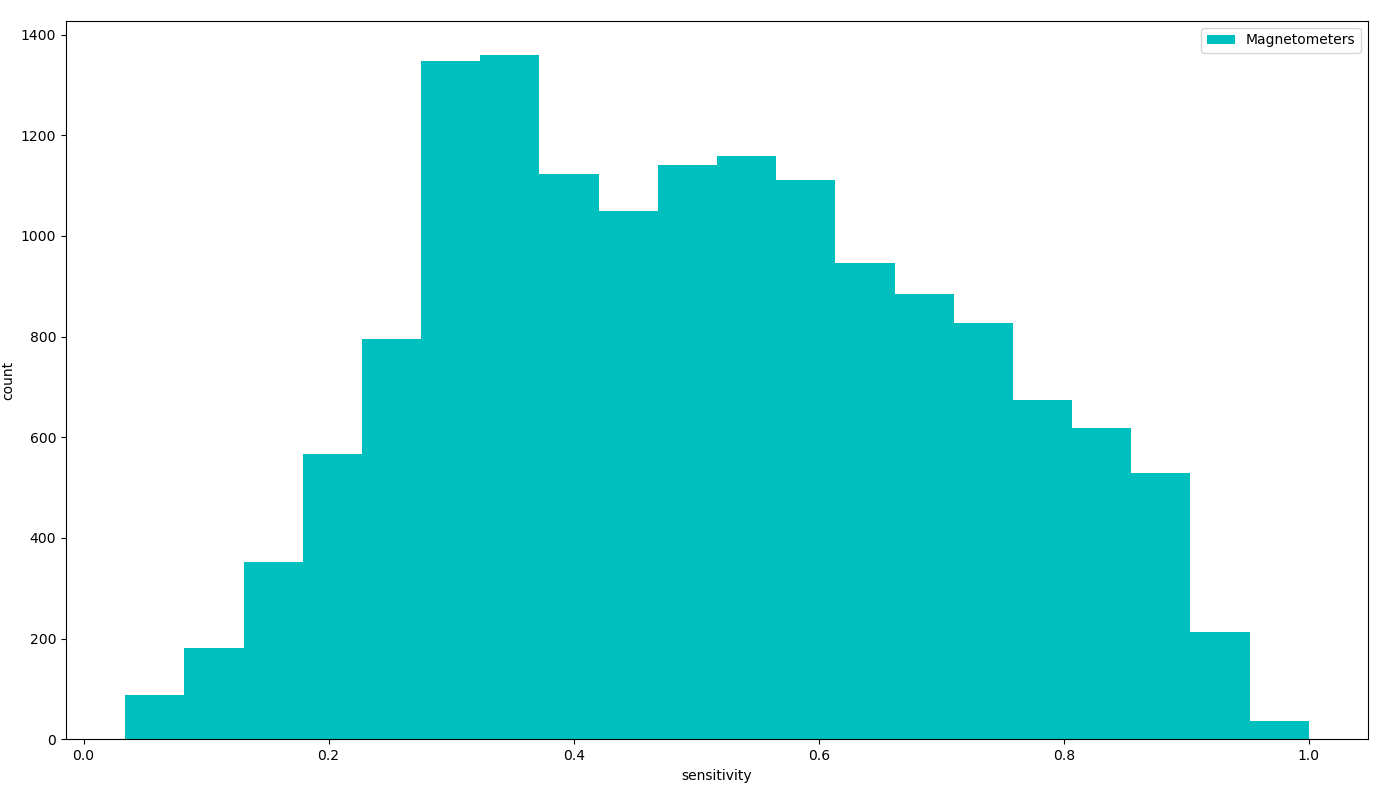
\includegraphics[width=\linewidth]{pictures/HISTmeg1.png}
             %\caption{\tiny RDF Shema (RDFS) graph}
            \label{fig:rdfs_graph}
        \end{subfigure}
       % \caption{\scriptsize Example of RDF graph and RDFS graph}
    \end{figure}

  
\end{frame}




%----------------------------------------------
\section{}
\begin{frame}
 \frametitle{MEG-Lambda min}
  

 	\begin{figure}[h]
        \begin{subfigure}[h]{0.53\linewidth} 
            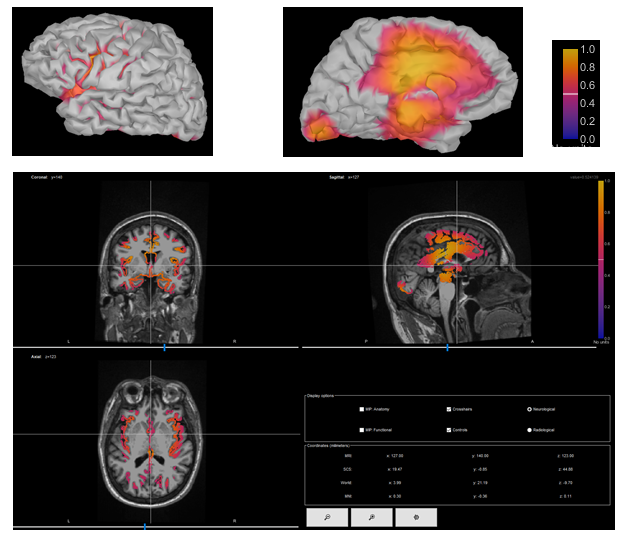
\includegraphics[width=\linewidth]{pictures/meg1}
           %  \caption{\tiny RDF graph}
            \label{fig:rdf_graph}
        \end{subfigure}       
        \begin{subfigure}[h]{0.45\linewidth} 
            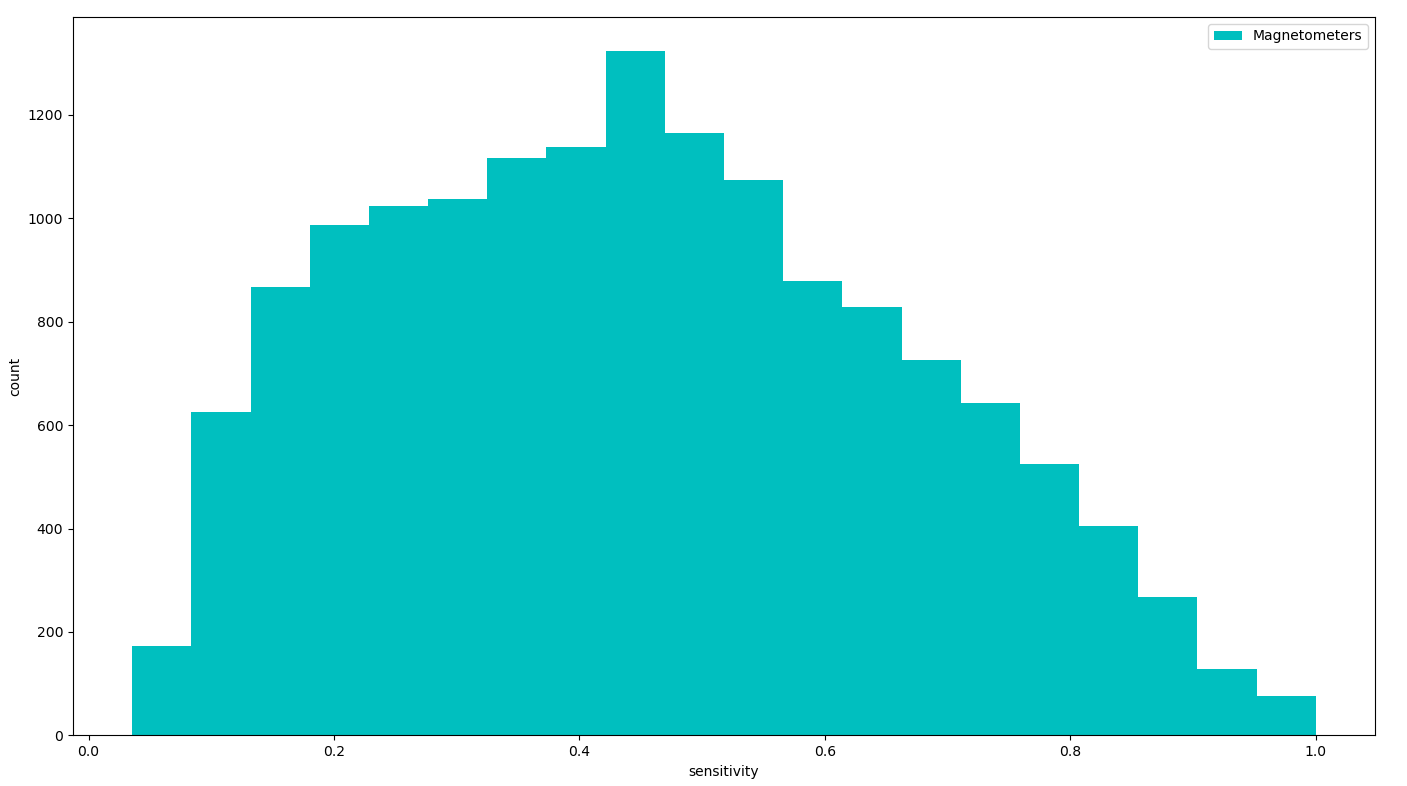
\includegraphics[width=\linewidth]{pictures/HISTmeg2.png}
           %  \caption{\tiny RDF Shema (RDFS) graph}
            \label{fig:rdfs_graph}
        \end{subfigure}
       % \caption{\scriptsize Example of RDF graph and RDFS graph}
    \end{figure}

  
\end{frame}

% ------------------------------------------------------------------------------------------------





%------------------

\section{}
\begin{frame}
 \frametitle{OPMX Lambda max}
  

 	\begin{figure}[h]
        \begin{subfigure}[h]{0.53\linewidth} 
            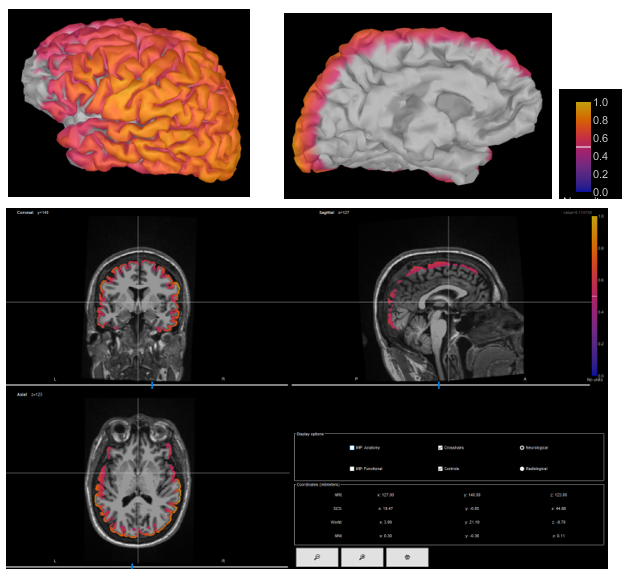
\includegraphics[width=\linewidth]{pictures/OPMX1}
            % \caption{\tiny RDF graph}
            \label{fig:rdf_graph}
        \end{subfigure}       
        \begin{subfigure}[h]{0.45\linewidth} 
            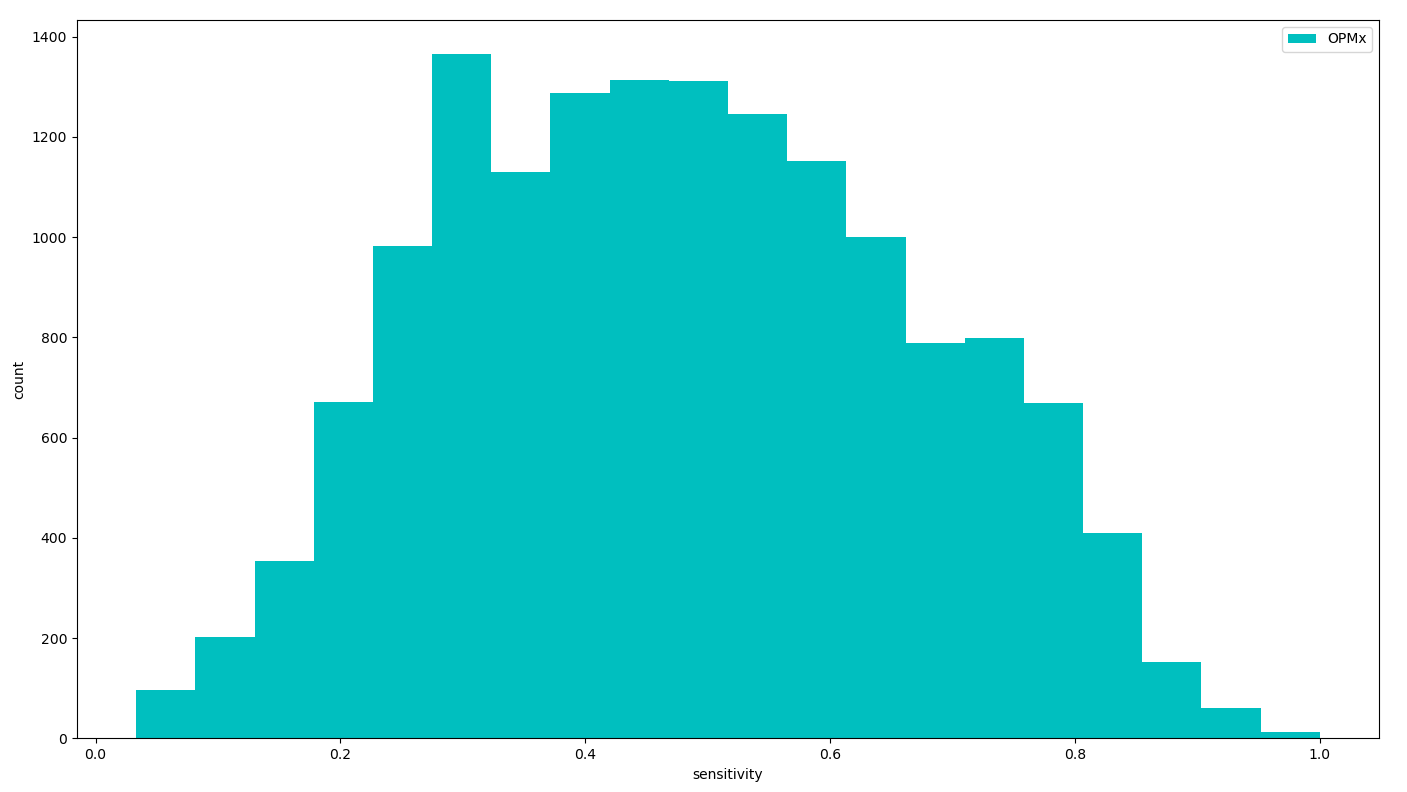
\includegraphics[width=\linewidth]{pictures/opmx0}
           %  \caption{\tiny RDF Shema (RDFS) graph}
            \label{fig:rdfs_graph}
        \end{subfigure}
       % \caption{\scriptsize Example of RDF graph and RDFS graph}
    \end{figure}

  
\end{frame}

%---------

\section{}
\begin{frame}
 \frametitle{OPMX Lambda2}
  

 	\begin{figure}[h]
        \begin{subfigure}[h]{0.53\linewidth} 
            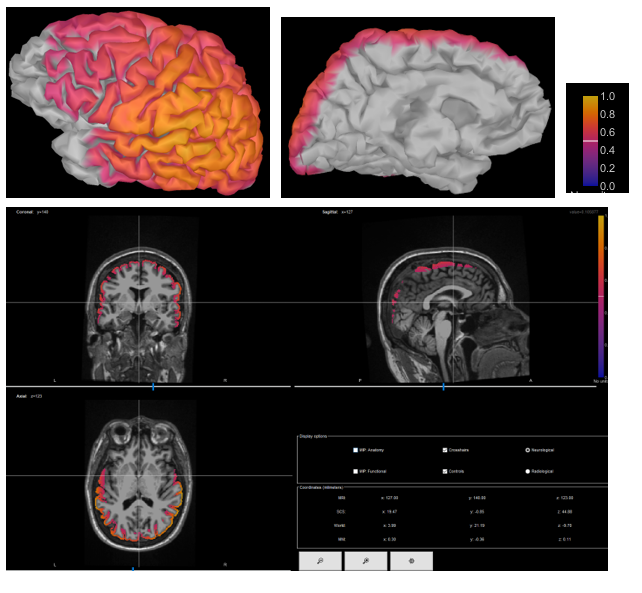
\includegraphics[width=\linewidth]{pictures/OPMX2}
           %  \caption{\tiny RDF graph}
            \label{fig:rdf_graph}
        \end{subfigure}       
        \begin{subfigure}[h]{0.45\linewidth} 
            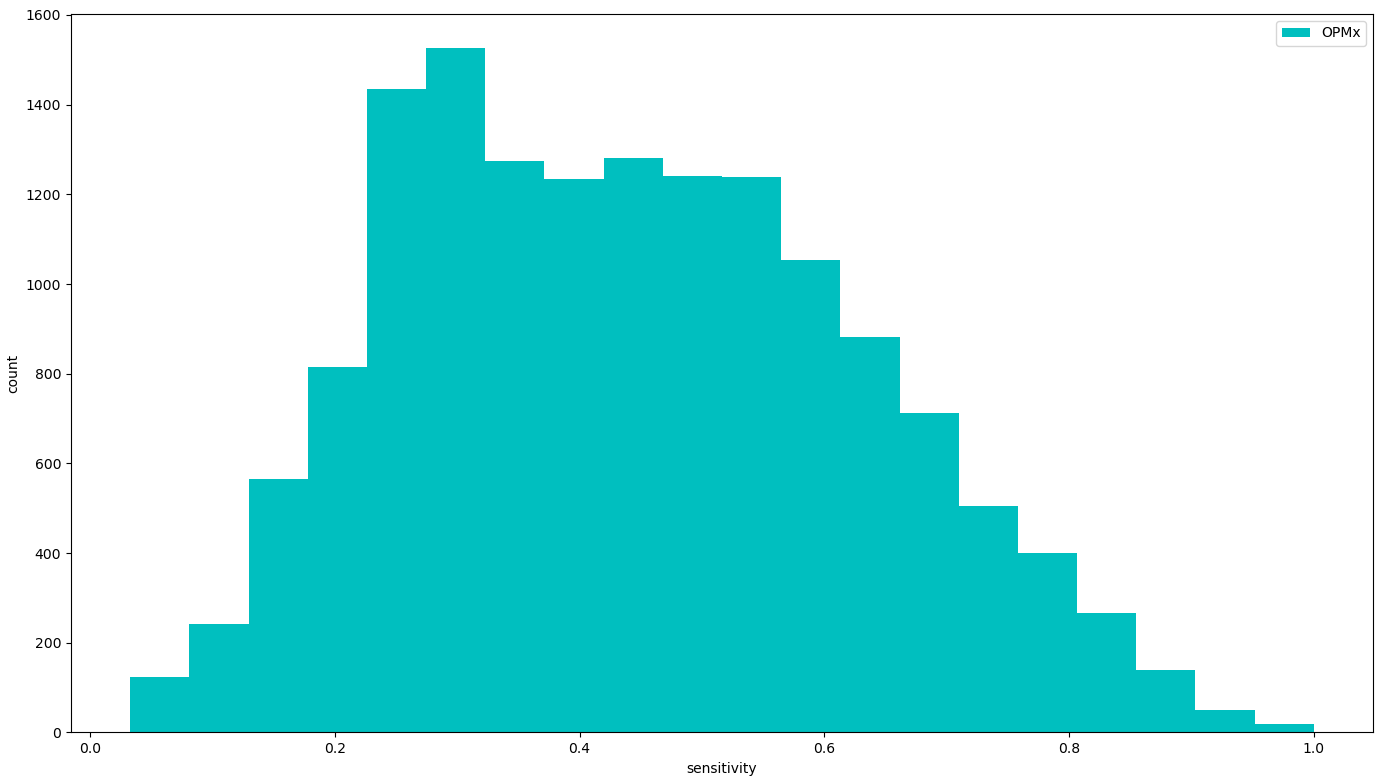
\includegraphics[width=\linewidth]{pictures/opmx1}
           %  \caption{\tiny RDF Shema (RDFS) graph}
            \label{fig:rdfs_graph}
        \end{subfigure}
       % \caption{\scriptsize Example of RDF graph and RDFS graph}
    \end{figure}

  
\end{frame}

%---------

\section{}
\begin{frame}
 \frametitle{OPMX Lambda min}
  

 	\begin{figure}[h]
        \begin{subfigure}[h]{0.53\linewidth} 
            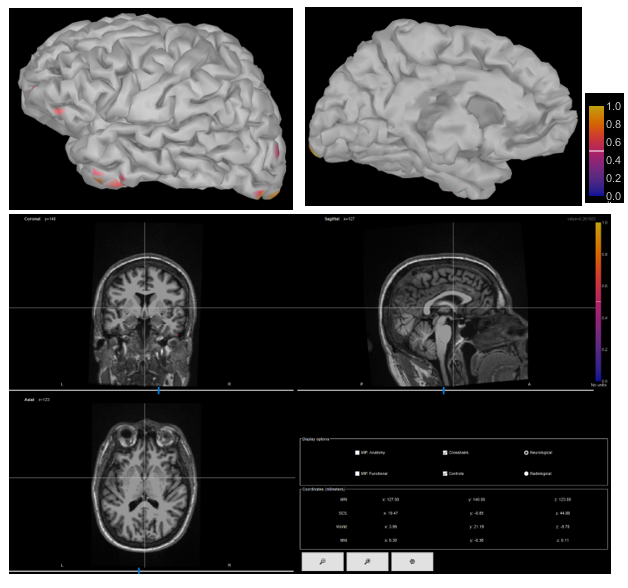
\includegraphics[width=\linewidth]{pictures/OPMX3}
          %  \caption{\tiny RDF graph}
            \label{fig:rdf_graph}
        \end{subfigure}       
        \begin{subfigure}[h]{0.45\linewidth} 
            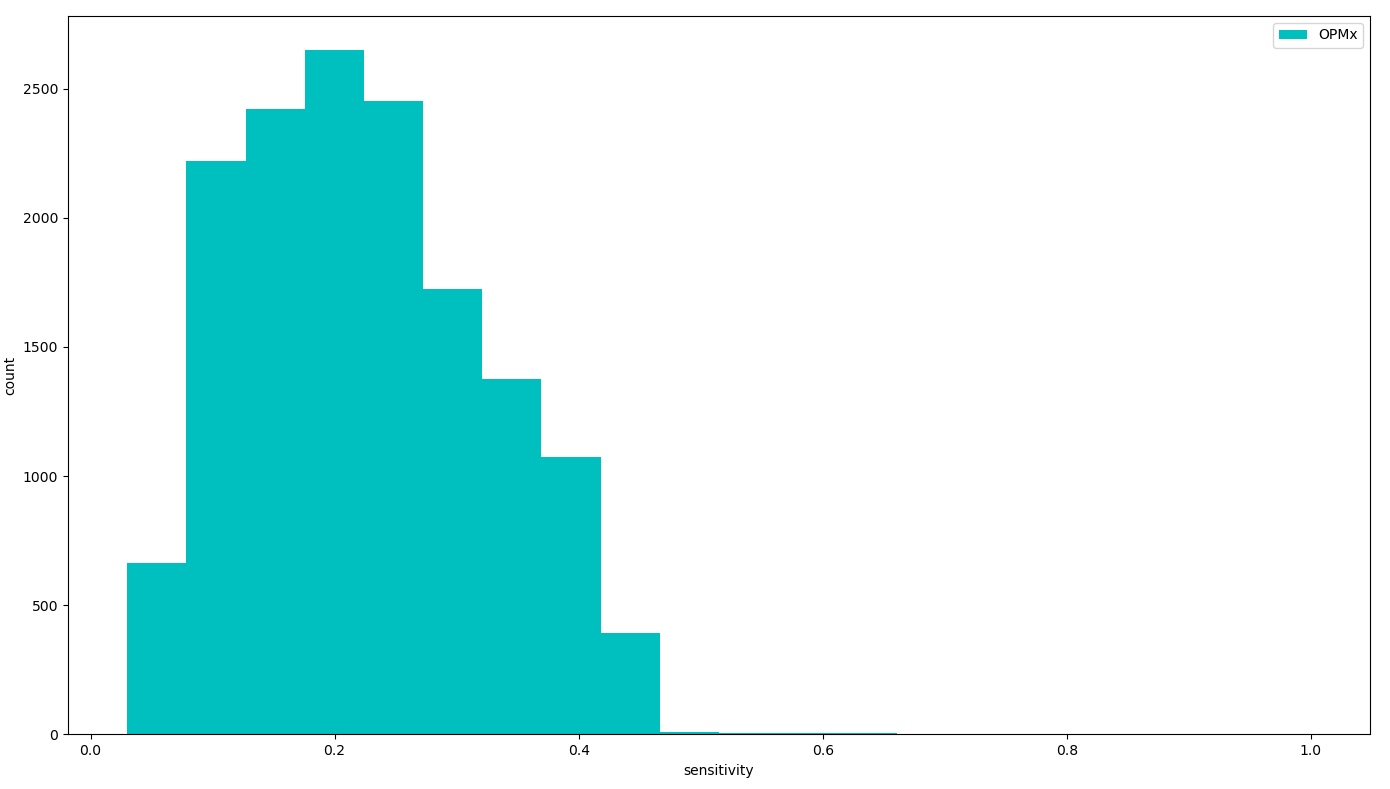
\includegraphics[width=\linewidth]{pictures/opmx2}
            %\caption{\tiny RDF Shema (RDFS) graph}
            \label{fig:rdfs_graph}
        \end{subfigure}
       % \caption{\scriptsize Example of RDF graph and RDFS graph}
    \end{figure}

  
\end{frame}


%---------

\section{}
\begin{frame}
 \frametitle{OPMy Lambda max}
  

 	\begin{figure}[h]
        \begin{subfigure}[h]{0.53\linewidth} 
            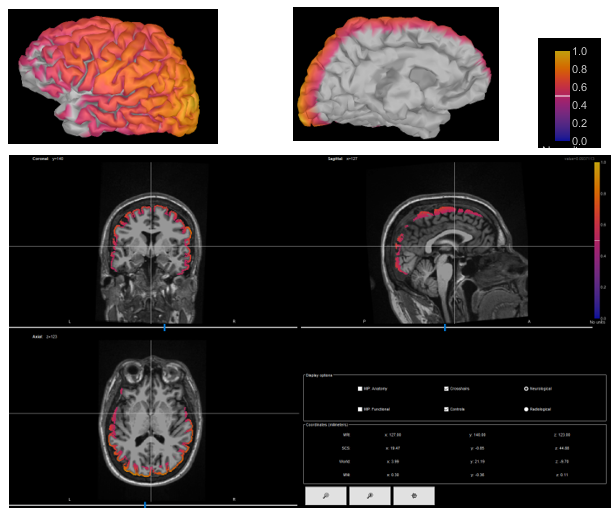
\includegraphics[width=\linewidth]{pictures/OPMY1}
           % \caption{\tiny RDF graph}
            \label{fig:rdf_graph}
        \end{subfigure}       
        \begin{subfigure}[h]{0.45\linewidth} 
            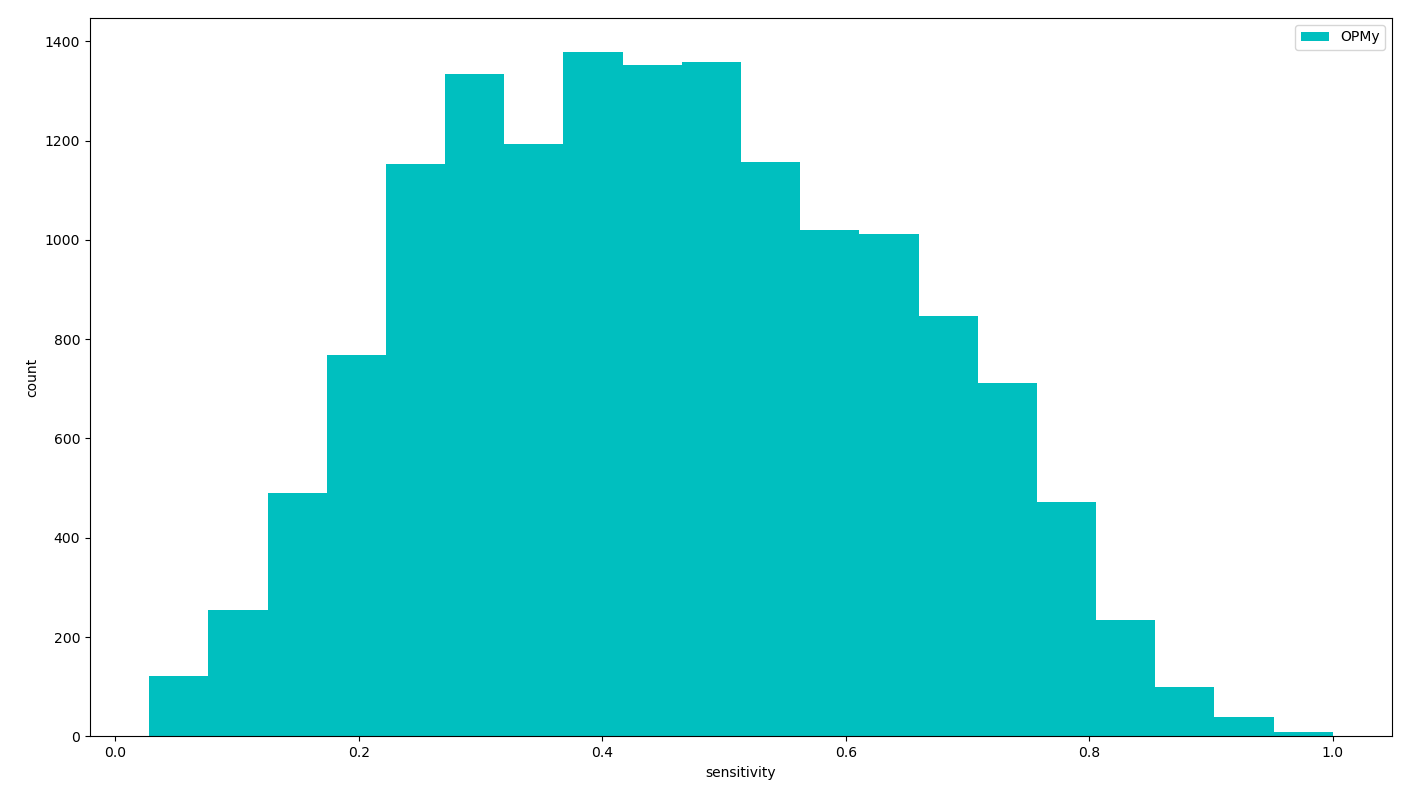
\includegraphics[width=\linewidth]{pictures/HISTopmy0}
           % \caption{\tiny RDF Shema (RDFS) graph}
            \label{fig:rdfs_graph}
        \end{subfigure}
       % \caption{\scriptsize Example of RDF graph and RDFS graph}
    \end{figure}

  
\end{frame}


%---------

\section{}
\begin{frame}
 \frametitle{OPMy Lambda2}
  

 	\begin{figure}[h]
        \begin{subfigure}[h]{0.53\linewidth} 
            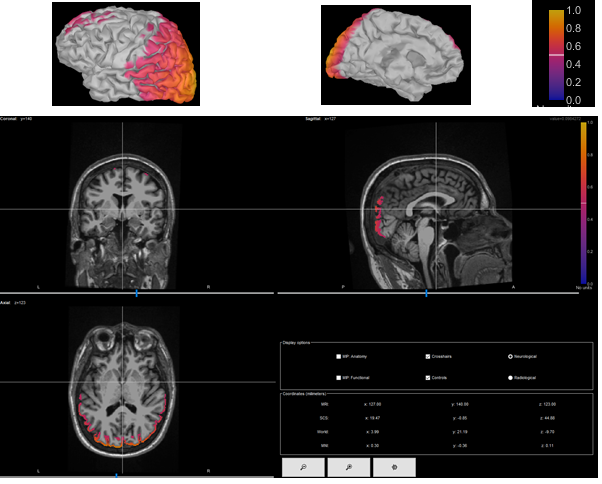
\includegraphics[width=\linewidth]{pictures/OPMY2}
          %  \caption{\tiny RDF graph}
            \label{fig:rdf_graph}
        \end{subfigure}       
        \begin{subfigure}[h]{0.45\linewidth} 
            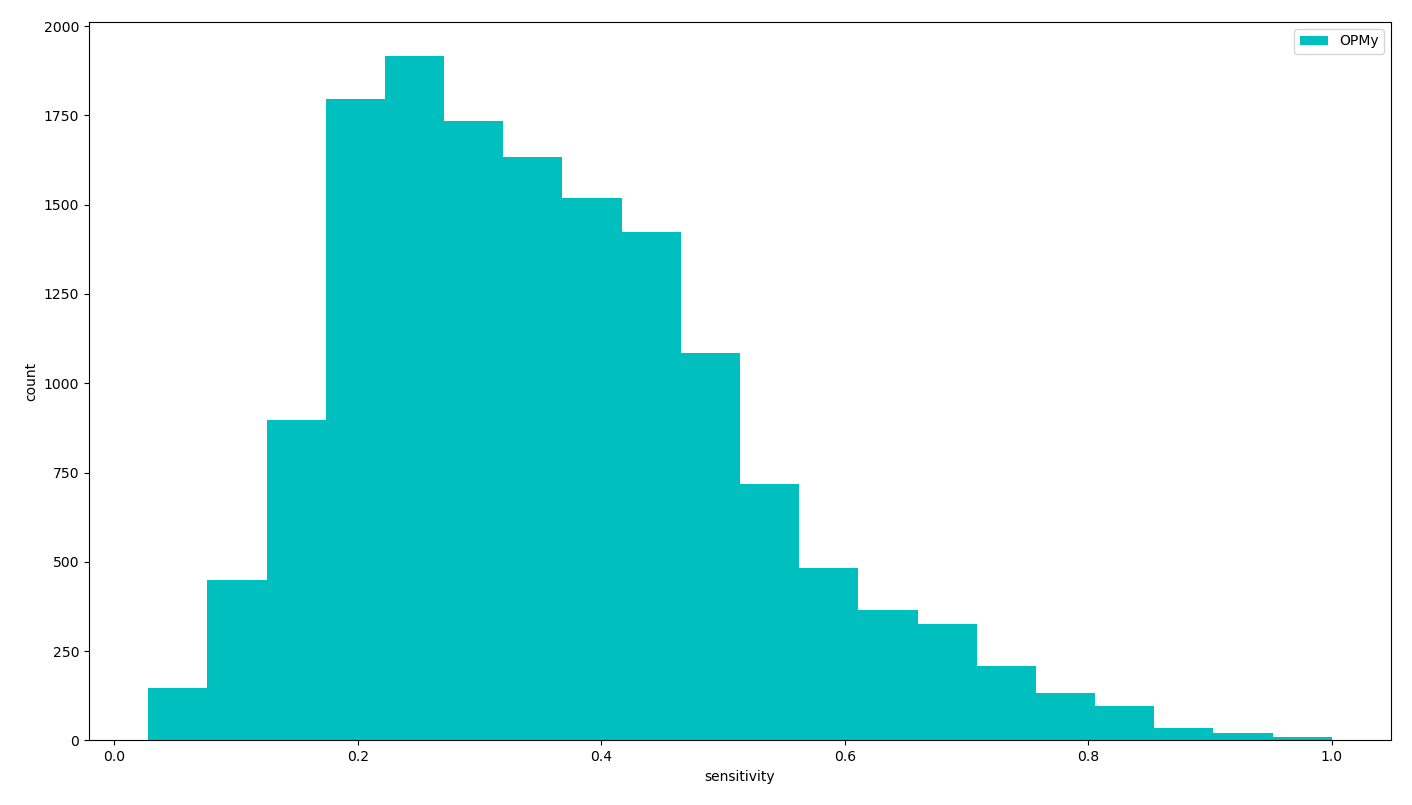
\includegraphics[width=\linewidth]{pictures/HISTopmy1}
            %\caption{\tiny RDF Shema (RDFS) graph}
            \label{fig:rdfs_graph}
        \end{subfigure}
       % \caption{\scriptsize Example of RDF graph and RDFS graph}
    \end{figure}

  
\end{frame}
%---------

\section{}
\begin{frame}
 \frametitle{OPMy Lambda min}
  

 	\begin{figure}[h]
        \begin{subfigure}[h]{0.53\linewidth} 
            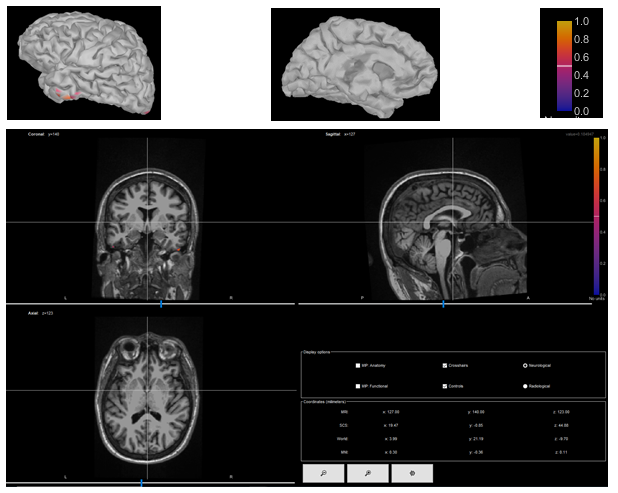
\includegraphics[width=\linewidth]{pictures/OPMY3}
          %  \caption{\tiny RDF graph}
            \label{fig:rdf_graph}
        \end{subfigure}       
        \begin{subfigure}[h]{0.45\linewidth} 
            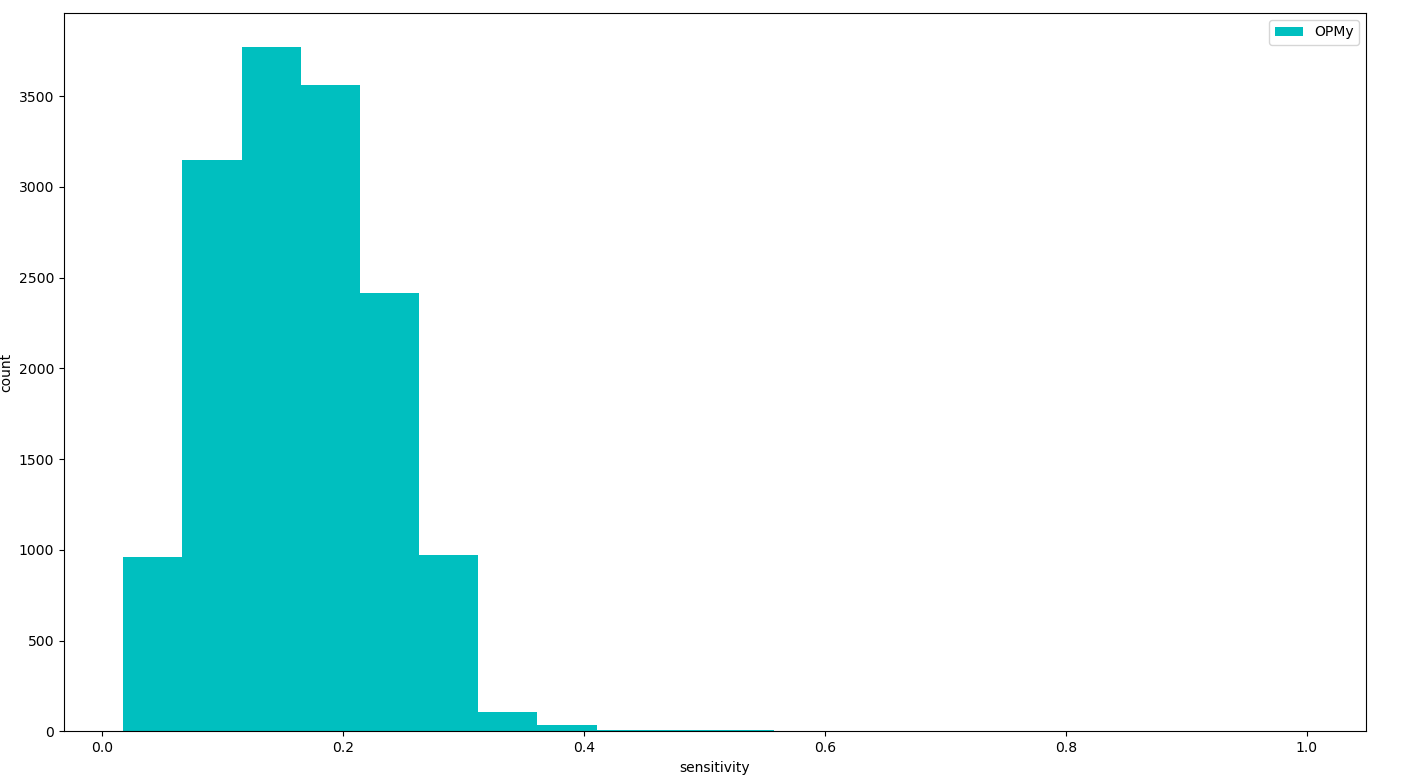
\includegraphics[width=\linewidth]{pictures/HISTopmy2}
           % \caption{\tiny RDF Shema (RDFS) graph}
            \label{fig:rdfs_graph}
        \end{subfigure}
       % \caption{\scriptsize Example of RDF graph and RDFS graph}
    \end{figure}

  
\end{frame}

\end{document}
